%%%%%%%%%%%%%%%%%%%%%%%%%%%%%%%%%%%%%%%%%%%%%%%%%%%%%%%%%%%%%%%%%%%%%%%
%%%%%%%%%%%%%%%%%%%%%%%%%%%%%%%%%%%%%%%%%%%%%%%%%%%%%%%%%%%%%%%%%%%%%%%
%%%%%                                                                 %
%%%%%     04_wdt_implementation.tex                                   %
%%%%%                                                                 %
%%%%% Author:      Miguel Correa, Elio Wanner                         %
%%%%% Created:     17.03.2025                                         %
%%%%% Description: In here is the description of the hardware         %
%%%%%                                                                 %
%%%%%%%%%%%%%%%%%%%%%%%%%%%%%%%%%%%%%%%%%%%%%%%%%%%%%%%%%%%%%%%%%%%%%%%
%%%%%%%%%%%%%%%%%%%%%%%%%%%%%%%%%%%%%%%%%%%%%%%%%%%%%%%%%%%%%%%%%%%%%%%

\chapter{Hardware Architecture}
This chapter describes the hardware architecture of the Watchdog Timer that we implemented in the Croc SoC.
In the different sections we talk about different implementations with different features and complexities.

\section{Simple Watchdog Timer}
\subsection{Hardware implementation}
The first implementation of the Watchdog Timer is the simplest one we could imagine. 
As shown in Figure \ref{fig:simple_WDT}, the WDT is composed of
very few components. The main component is the counter, which is
incremented every clock cycle and implemented as a flip-flop. The counter is connected to a comparator
that checks if the counter has reached a certain value. If the counter
reaches the value, the comparator will trigger a reset signal that will
reset the system. Otherwise, we keep incrementing the counter. As soon as we get
a kick signal, the counter is reset to zero.

\begin{figure}[h]
\centering
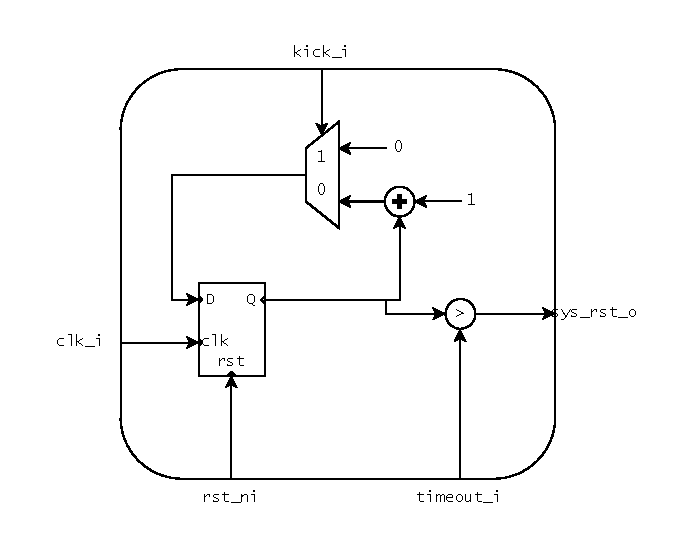
\includegraphics[width=0.7\textwidth]{./figures/simple_WDT}
\caption{Simple Watchdog Timer Architecture}
\label{fig:simple_WDT}
\end{figure}

\subsection{Tests and Results}
Explain how we did the tests (python files to generate stimuli + expected then compare), show figure.
Explain that the results were always good at the end.

\subsection{Conclusion}
Explain that thanks to our approach we found that the watchdog works fine, so if a future problem would come it would come from the wrapper.

\section{Watchdog Wrapper}
\subsection{Hardware implementation}
Add a graph of the watchdog wrapper, and maybe a figure of how it connects to the OBI protocol.

\subsection{Tests and Results}
We checked the functionality of our wrapper by running a helloword.c wich sets the timeout value and sends periodic kicks befor getting stuck in an impossible task. Our watchdog was successfully set thanks to the correctness of the wrapper and it allowed us to reset the program. We also checked the VCD to see if we could find any anormalities, but our wrapper respects OBI protocol :) .
